\chapter{Desenvolvimento}

Esta seção tem por propósito apresentar a pesquisa elaborada a respeito dos estilos arquiteturais
abordados no presente trabalho. O escopo deste capítulo abrangerá o estudo feito sobre os objetos de
análise referidos na \autoref{sec:ObjetosDeAnalise}, os aspectos levantados sobre cada
arquitetura e análise comparativa realizada.

As seções estão dispostas em:

  \begin{enumerate}
    \item \textbf{Síntese das perspectivas teóricas} síntese a respeitos das informações
        coletadas nos referenciais teóricos sobre cada arquitetura;
    \item \textbf{Análise dos casos de estudo} detalhamento sobre as experiências de algumas empresas
    que optaram por fazer a migração de uma arquitetura monolítica para uma arquitetura de
    microsserviços ou vice-versa.
  \end{enumerate}

\section{Síntese das perspectivas teóricas}
\label{sinteses}

O presente tópico visa apresentar a síntese das perspectivas abordadas na \autoref{perspectivas} da
fundamentação teórica com o intuito de esclarecer os pontos chaves presentes em cada arquitetura.
Para tal, organizou-se os temas discutidos na fundamentação teórica no modelo do \autoref{modelo-sintese} 
apresentado na seção metodológica.

\subsection{Síntese da arquitetura monolítica}
\label{monoSintese}

\begin{quadro}
    \caption{Arquitetura monolítica - síntese sobre o domínio do problema\label{monolitico:sintese-dominio}}
    \begin{tabularx}{\linewidth}{ | p{5cm} | X | }
    \hline
    \textbf{A escolha de uma}       & arquitetura monolítica \\ \hline
    \textbf{sob a perspectiva}      & da problemática a ser resolvida \\ \hline
    \textbf{mediante o aspecto}     & de domínio sobre o problema \\ \hline
    \textbf{gera um impacto}        & positivo se o domínio sobre o contexto é baixo\\ \hline
    \textbf{devido à }              & arquitetura simplista \\ \hline
    % \textbf{contudo}                & \\ \hline
    % \textbf{consciente de que este aspecto tende a }          & \\ \hline
    \textbf{com base na}            & \autoref{Perspectivas:Problematica} \\ \hline
    \end{tabularx}
\end{quadro}

\begin{quadro}
    \caption{Arquitetura monolítica - síntese sobre o tamanho da aplicação\label{monolitico:sintese-tamanho}}
    \begin{tabularx}{\linewidth}{ | p{5cm} | X | }
    \hline
    \textbf{A escolha de uma}       & arquitetura monolítica \\ \hline
    \textbf{sob a perspectiva}      & da problemática a ser resolvida \\ \hline
    \textbf{mediante o aspecto}     & do tamanho planejado para a aplicação \\ \hline
    \textbf{gera um impacto}        & positivo se a aplicação é pequena \\ \hline
    \textbf{devido à }              & arquitetura simplista e a simplicidade dos processos operacionais\\ \hline
    % \textbf{contudo}                & \\ \hline
    % \textbf{consciente de que este aspecto tende a} & \\ \hline
    \textbf{com base na}            & \autoref{Perspectivas:Problematica} \\ \hline
    \end{tabularx}
\end{quadro}

\begin{quadro}
    \caption{Arquitetura monolítica - síntese sobre os recursos financeiros\label{monolitico:sintese-financeiros}}
    \begin{tabularx}{\linewidth}{ | p{5cm} | X | }
    \hline
    \textbf{A escolha de uma}       & arquitetura monolítica \\ \hline
    \textbf{sob a perspectiva}      & recursos necessários \\ \hline
    \textbf{mediante o aspecto}     & de recursos financeiros \\ \hline
    \textbf{gera um impacto}        & baixo custo \\ \hline
    \textbf{devido à }              & arquitetura simplista e a simplicidade dos processos operacionais\\ \hline
    % \textbf{contudo}                & \\ \hline
    % \textbf{consciente de que este aspecto tende a} & \\ \hline
    \textbf{com base na}            & \autoref{Perspectivas:recursosFinanceiros} \\ \hline
    \end{tabularx}
\end{quadro}

\begin{quadro}
    \caption{Arquitetura monolítica - síntese sobre os recursos humanos\label{monolitico:sintese-humanos}}
    \begin{tabularx}{\linewidth}{ | p{5cm} | X | }
    \hline
    \textbf{A escolha de uma}       & arquitetura monolítica \\ \hline
    \textbf{sob a perspectiva}      & recursos necessários \\ \hline
    \textbf{mediante o aspecto}     & de recursos humanos \\ \hline
    \textbf{gera um impacto}        & não necessitar de expertise sobre as tecnologias \\ \hline
    \textbf{devido à }              & arquitetura simplista e a simplicidade dos processos operacionais\\ \hline
    % \textbf{contudo}                & \\ \hline
    % \textbf{consciente de que este aspecto tende a} & \\ \hline
    \textbf{com base na}            & \autoref{Perspectivas:recursosHumanos} \\ \hline
    \end{tabularx}
\end{quadro}

\begin{quadro}
    \caption{Arquitetura monolítica - síntese sobre esforço e tempo inicial\label{monolitico:sintese-esforco}}
    \begin{tabularx}{\linewidth}{ | p{5cm} | X | }
    \hline
    \textbf{A escolha de uma}       & arquitetura monolítica \\ \hline
    \textbf{sob a perspectiva}      & recursos necessários \\ \hline
    \textbf{mediante o aspecto}     & esforço e tempo inicial \\ \hline
    \textbf{gera um impacto}        & baixo esforço inicial e rápido lançamento no mercado \\ \hline
    \textbf{devido à }              & arquitetura simplista e a simplicidade dos processos operacionais\\ \hline
    % \textbf{contudo}                & \\ \hline
    % \textbf{consciente de que este aspecto tende a} & \\ \hline
    \textbf{com base na}            & \autoref{effortsAndTime} \\ \hline
    \end{tabularx}
\end{quadro}

\begin{quadro}
    \caption{Arquitetura monolítica - síntese sobre escalabilidade\label{monolitico:sintese-escalabilidade}}
    \begin{tabularx}{\linewidth}{ | p{5cm} | X | }
    \hline
    \textbf{A escolha de uma}       & arquitetura monolítica \\ \hline
    \textbf{sob a perspectiva}      & de características arquiteturais \\ \hline
    \textbf{mediante o aspecto}     & da escalabilidade \\ \hline
    \textbf{gera um impacto}        & de escalabilidade limitada \\ \hline
    \textbf{devido à }              & baixa modularidade da arquitetura \\ \hline
    % \textbf{contudo}                & \\ \hline
    % \textbf{consciente de que este aspecto tende a} & \\ \hline
    \textbf{com base na}            & \autoref{pers:escalabilidade} \\ \hline
    \end{tabularx}
\end{quadro}

\begin{quadro}
    \caption{Arquitetura monolítica - síntese sobre tolerância a falhas\label{monolitico:sintese-tolerancia}}
    \begin{tabularx}{\linewidth}{ | p{5cm} | X | }
    \hline
    \textbf{A escolha de uma}       & arquitetura monolítica \\ \hline
    \textbf{sob a perspectiva}      & de características arquiteturais \\ \hline
    \textbf{mediante o aspecto}     & de tolerância a falhas \\ \hline
    \textbf{gera um impacto}        & não possui tolerância a falhas \\ \hline
    \textbf{devido à }              & a existência de um único ponto de falha em toda a arquitetura \\ \hline
    % \textbf{contudo}                & \\ \hline
    % \textbf{consciente de que este aspecto tende a} & \\ \hline
    \textbf{com base na}            & \autoref{pers:tolerancia} \\ \hline
    \end{tabularx}
\end{quadro}

\begin{quadro}
    \caption{Arquitetura monolítica - síntese sobre confiabilidade\label{monolitico:sintese-confiabilidade}}
    \begin{tabularx}{\linewidth}{ | p{5cm} | X | }
    \hline
    \textbf{A escolha de uma}       & arquitetura monolítica \\ \hline
    \textbf{sob a perspectiva}      & de características arquiteturais \\ \hline
    \textbf{mediante o aspecto}     & de confiabilidade do sistema \\ \hline
    \textbf{gera um impacto}        & alta confiabilidade \\ \hline
    % \textbf{devido à }              & \\ \hline
    \textbf{contudo}                & é preciso lidar com a testabilidade do sistema\\ \hline
    \textbf{consciente de que este aspecto tende a} & decair a medida que a base de código aumenta \\ \hline
    \textbf{com base na}            & \autoref{pers:confiabilidade} \\ \hline
    \end{tabularx}
\end{quadro}

\begin{quadro}
    \caption{Arquitetura monolítica - síntese sobre performance\label{monolitico:sintese-performance}}
    \begin{tabularx}{\linewidth}{ | p{5cm} | X | }
    \hline
    \textbf{A escolha de uma}       & arquitetura monolítica \\ \hline
    \textbf{sob a perspectiva}      & de características arquiteturais \\ \hline
    \textbf{mediante o aspecto}     & de performance do sistema \\ \hline
    \textbf{gera um impacto}        & baixa performance \\ \hline
    \textbf{devido à }              & arquitetura simplista \\ \hline
    % \textbf{contudo}                & \\ \hline
    % \textbf{consciente de que este aspecto tende a} & \\ \hline
    \textbf{com base na}            & \autoref{pers:performance} \\ \hline
    \end{tabularx}
\end{quadro}

\begin{quadro}
    \caption{Arquitetura monolítica - síntese sobre o processo de \textit{deploy}\label{monolitico:sintese-deploy}}
    \begin{tabularx}{\linewidth}{ | p{5cm} | X | }
    \hline
    \textbf{A escolha de uma}       & arquitetura monolítica \\ \hline
    \textbf{sob a perspectiva}      & de manutenibilidade \\ \hline
    \textbf{mediante o aspecto}     & de implantação do sistema \\ \hline
    \textbf{gera um impacto}        & de fácil implantação \\ \hline
    \textbf{devido à }              & arquitetura simplista \\ \hline
    \textbf{contudo}                & é preciso lidar com a crescente base de código\\ \hline
    \textbf{consciente de que este aspecto tende a} & decair a medida que a base de código fica maior \\ \hline
    \textbf{com base na}            & \autoref{pers:deploy} \\ \hline
    \end{tabularx}
\end{quadro}

\begin{quadro}
    \caption{Arquitetura monolítica - síntese da testabilidade\label{monolitico:sintese-testabilidade}}
    \begin{tabularx}{\linewidth}{ | p{5cm} | X | }
    \hline
    \textbf{A escolha de uma}       & arquitetura monolítica \\ \hline
    \textbf{sob a perspectiva}      & de manutenibilidade \\ \hline
    \textbf{mediante o aspecto}     & de testabilidade do sistema \\ \hline
    \textbf{gera um impacto}        & de facilidade para realizar testes \\ \hline
    \textbf{devido à }              & arquitetura simplista \\ \hline
    \textbf{contudo}                & é preciso lidar com a crescente complexidade\\ \hline
    \textbf{consciente de que este aspecto tende a} & decair a medida que a complexidade do sistema aumenta \\ \hline
    \textbf{com base na}            & \autoref{testabilidade} \\ \hline
    \end{tabularx}
\end{quadro}

\begin{quadro}
    \caption{Arquitetura monolítica - síntese da comunicação\label{monolitico:sintese-comunicacao}}
    \begin{tabularx}{\linewidth}{ | p{5cm} | X | }
    \hline
    \textbf{A escolha de uma}       & arquitetura monolítica \\ \hline
    \textbf{sob a perspectiva}      & de manutenibilidade \\ \hline
    \textbf{mediante o aspecto}     & de comunicação entre os times \\ \hline
    \textbf{gera um impacto}        & negativo \\ \hline
    \textbf{devido aos}              & times segregados por domínio tecnológico \\ \hline
    % \textbf{contudo}                & é preciso lidar com a comunicação entre diferentes áreas\\ \hline
    % \textbf{consciente de que este aspecto tende a} & decair a medida que a complexidade do sistema aumenta \\ \hline
    \textbf{com base na}            & \autoref{pers:comunicacao} \\ \hline
    \end{tabularx}
\end{quadro}

\begin{quadro}
    \caption{Arquitetura monolítica - síntese da heterogeneidade das tecnologias\label{monolitico:sintese-heterogeneidade}}
    \begin{tabularx}{\linewidth}{ | p{5cm} | X | }
    \hline
    \textbf{A escolha de uma}       & arquitetura monolítica \\ \hline
    \textbf{sob a perspectiva}      & de evolucionabilidade \\ \hline
    \textbf{mediante o aspecto}     & de heterogeneidade das tecnologias \\ \hline
    \textbf{gera um impacto}        & de heterogeneidade limitada \\ \hline
    \textbf{devido ao}              & modelo arquitetural com alto acoplamento \\ \hline
    % \textbf{contudo}                & é preciso lidar com a comunicação entre diferentes áreas\\ \hline
    % \textbf{consciente de que este aspecto tende a} & decair a medida que a complexidade do sistema aumenta \\ \hline
    \textbf{com base na}            & \autoref{pers:heterogeneidade} \\ \hline
    \end{tabularx}
\end{quadro}

\begin{quadro}
    \caption{Arquitetura monolítica - síntese sobre complexidade do sistema\label{monolitico:sintese-complexidade}}
    \begin{tabularx}{\linewidth}{ | p{5cm} | X | }
    \hline
    \textbf{A escolha de uma}       & arquitetura monolítica \\ \hline
    \textbf{sob a perspectiva}      & de evolucionabilidade \\ \hline
    \textbf{mediante o aspecto}     & da complexidade do sistema \\ \hline
    \textbf{gera um impacto}        & de baixa complexidade \\ \hline
    \textbf{devido ao}              & arquitetura simplista \\ \hline
    \textbf{contudo}                & é preciso lidar com o acoplamento do código \\ \hline
    \textbf{consciente de que este aspecto tende a} & crescer a medida que ao crescimento da base de código\\ \hline
    \textbf{com base na}            & \autoref{pers:heterogeneidade} \\ \hline
    \end{tabularx}
\end{quadro}

\newpage

A \autoref{fig:SinteseMono} visa ilustrar um resumo dos pontos destacados com base na síntese do
referêncial teórico. Nela podemos observar de verde os fatores positivos da arquitetura, de amarelo
os fatores negativos e de vermelho os fatores que inicialmente são positivos dentro do modelo
arquitetural mas que tendem a decair a medida que a base de código aumenta.

É importante ter em mente que os fatores marcados como negativo, cor amarela, são características da
arquitetura monolítica, com as quais a equipe de software ao optar por este modelo arquitetural vai
ter que lhe dar conscientemente que estes problemas existem. Já os fatores marcados com a cor
vermelha, que tendem a cair, são mais traiçoeiros, de forma que inicialmente eles não são um
problema, pelo contrário, eles são algo positivo quando se tem um monolítico novo, porém a medida que
a base de código cresce eles tendem a se tornar um problema que se instala na arquitetura sem a
equipe de \gls{TI} perceba.

\begin{figure}[h]
  \centering
  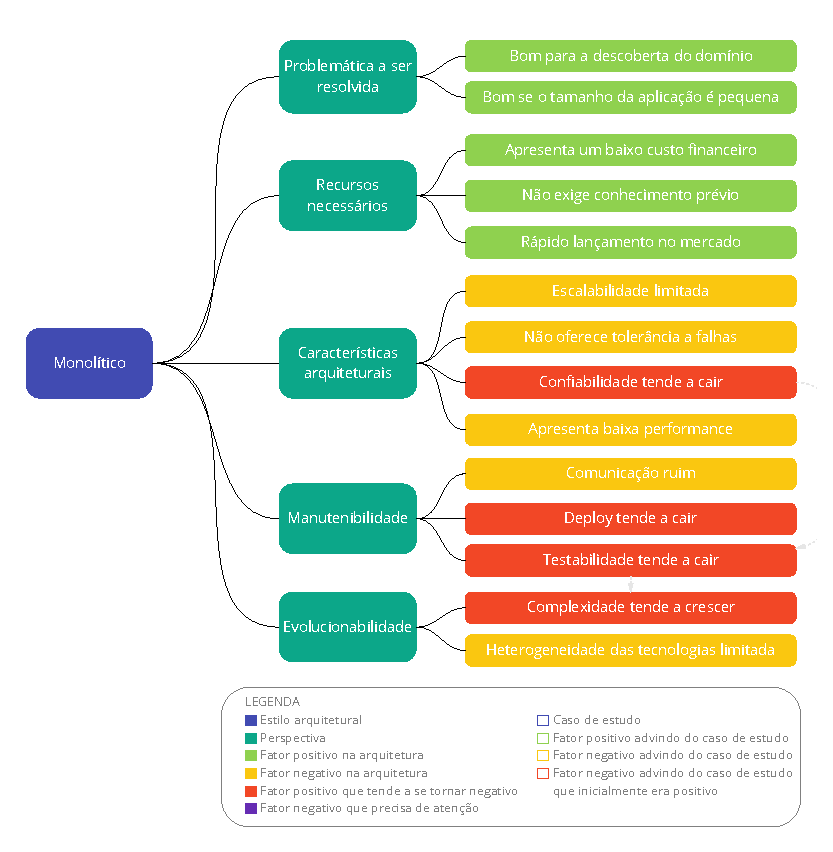
\includegraphics[keepaspectratio=true,scale=1]{figuras/sintese-monolitico.eps}
  \caption{Mapa mental do processo de síntese realizado sobre a arquitetura monolítica\label{fig:SinteseMono}}
\end{figure}

%%%%%%%%%%%%%%%%%%%%%%%%%%%%%%%%%%%%%%%%%%%%%%%%%%%%%%%%%%%%%%%%%%%%%%%%%%%%%%%%%%%%%%%%%%

\newpage
\subsection{Síntese da arquitetura de microsserviços}

\begin{quadro}
    \caption{Arquitetura de microsserviços - síntese sobre o domínio do problema\label{microsservicos:sintese-dominio}}
    \begin{tabularx}{\linewidth}{ | p{5cm} | X | }
    \hline
    \textbf{A escolha de uma}       & arquitetura de microsserviços \\ \hline
    \textbf{sob a perspectiva}      & da problemática a ser resolvida \\ \hline
    \textbf{mediante o aspecto}     & de domínio sobre o problema \\ \hline
    \textbf{gera um impacto}        & de necessidade de domínio sobre o contexto\\ \hline
    \textbf{devido à }              & definição dos limites que impacta toda a arquitetura \\ \hline
    % \textbf{contudo}                & \\ \hline
    % \textbf{consciente de que este aspecto tende a }          & \\ \hline
    \textbf{com base na}            & \autoref{Perspectivas:Problematica} \\ \hline
    \end{tabularx}
\end{quadro}

\begin{quadro}
    \caption{Arquitetura de microsserviços - síntese sobre o tamanho da aplicação\label{microsservicos:sintese-tamanho}}
    \begin{tabularx}{\linewidth}{ | p{5cm} | X | }
    \hline
    \textbf{A escolha de uma}       & arquitetura de microsserviços \\ \hline
    \textbf{sob a perspectiva}      & da problemática a ser resolvida \\ \hline
    \textbf{mediante o aspecto}     & do tamanho planejado para a aplicação \\ \hline
    \textbf{gera um impacto}        & de custo muito alto para aplicações pequenas \\ \hline
    \textbf{devido ao}              & custo muito alto de implementação e manutenção\\ \hline
    % \textbf{contudo}                & \\ \hline
    % \textbf{consciente de que este aspecto tende a} & \\ \hline
    \textbf{com base na}            & \autoref{Perspectivas:Problematica} \\ \hline
    \end{tabularx}
\end{quadro}

\begin{quadro}
    \caption{Arquitetura de microsserviços - síntese sobre os recursos financeiros\label{microsservicos:sintese-financeiros}}
    \begin{tabularx}{\linewidth}{ | p{5cm} | X | }
    \hline
    \textbf{A escolha de uma}       & arquitetura de microsserviços \\ \hline
    \textbf{sob a perspectiva}      & recursos necessários \\ \hline
    \textbf{mediante o aspecto}     & de recursos financeiros \\ \hline
    \textbf{gera um impacto}        & alto custo \\ \hline
    \textbf{devido à }              & necessidade de mão de obra especializada, monitoramento, replicação...\\ \hline
    % \textbf{contudo}                & \\ \hline
    % \textbf{consciente de que este aspecto tende a} & \\ \hline
    \textbf{com base na}            & \autoref{Perspectivas:recursosFinanceiros} \\ \hline
    \end{tabularx}
\end{quadro}

\begin{quadro}
    \caption{Arquitetura de microsserviços - síntese sobre os recursos humanos\label{microsservicos:sintese-humanos}}
    \begin{tabularx}{\linewidth}{ | p{5cm} | X | }
    \hline
    \textbf{A escolha de uma}       & arquitetura de microsserviços \\ \hline
    \textbf{sob a perspectiva}      & recursos necessários \\ \hline
    \textbf{mediante o aspecto}     & de recursos humanos \\ \hline
    \textbf{gera um impacto}        & necessita de expertise sobre as tecnologias \\ \hline
    \textbf{devido à }              & complexidade da arquitetura \\ \hline
    % \textbf{contudo}                & \\ \hline
    % \textbf{consciente de que este aspecto tende a} & \\ \hline
    \textbf{com base na}            & \autoref{Perspectivas:recursosHumanos} \\ \hline
    \end{tabularx}
\end{quadro}

\begin{quadro}
    \caption{Arquitetura de microsserviços - síntese sobre esforço e tempo inicial\label{microsservicos:sintese-esforco}}
    \begin{tabularx}{\linewidth}{ | p{5cm} | X | }
    \hline
    \textbf{A escolha de uma}       & arquitetura de microsserviços \\ \hline
    \textbf{sob a perspectiva}      & recursos necessários \\ \hline
    \textbf{mediante o aspecto}     & esforço e tempo inicial \\ \hline
    \textbf{gera um impacto}        & alto esforço inicial e demorado lançamento no mercado \\ \hline
    \textbf{devido à }              & complexidade da arquitetura e a necessidade de automatizar todos os processos operacionais \\ \hline
    % \textbf{contudo}                & \\ \hline
    % \textbf{consciente de que este aspecto tende a} & \\ \hline
    \textbf{com base na}            & \autoref{effortsAndTime} \\ \hline
    \end{tabularx}
\end{quadro}

\begin{quadro}
    \caption{Arquitetura de microsserviços - síntese sobre escalabilidade\label{microsservicos:sintese-escalabilidade}}
    \begin{tabularx}{\linewidth}{ | p{5cm} | X | }
    \hline
    \textbf{A escolha de uma}       & arquitetura de microsserviços \\ \hline
    \textbf{sob a perspectiva}      & de características arquiteturais \\ \hline
    \textbf{mediante o aspecto}     & da escalabilidade \\ \hline
    \textbf{gera um impacto}        & de ser altamente escalável \\ \hline
    \textbf{devido à }              & alta modularidade e automatização dos processos \\ \hline
    % \textbf{contudo}                & \\ \hline
    % \textbf{consciente de que este aspecto tende a} & \\ \hline
    \textbf{com base na}            & \autoref{pers:escalabilidade} \\ \hline
    \end{tabularx}
\end{quadro}

\begin{quadro}
    \caption{Arquitetura de microsserviços - síntese sobre tolerância a falhas\label{microsservicos:sintese-tolerancia}}
    \begin{tabularx}{\linewidth}{ | p{5cm} | X | }
    \hline
    \textbf{A escolha de uma}       & arquitetura de microsserviços \\ \hline
    \textbf{sob a perspectiva}      & de características arquiteturais \\ \hline
    \textbf{mediante o aspecto}     & de tolerância a falhas \\ \hline
    \textbf{gera um impacto}        & alta tolerância \\ \hline
    \textbf{devido à }              & presença de vários pontos de falha, comprometendo apenas parcialmente a aplicação\\ \hline
    \textbf{contudo}                & é preciso lidar com a escalabilidade da rede \\ \hline
    % \textbf{consciente de que este aspecto tende a} & \\ \hline
    \textbf{com base na}            & \autoref{pers:tolerancia} \\ \hline
    \end{tabularx}
\end{quadro}

\begin{quadro}
    \caption{Arquitetura de microsserviços - síntese sobre confiabilidade\label{microsservicos:sintese-confiabilidade}}
    \begin{tabularx}{\linewidth}{ | p{5cm} | X | }
    \hline
    \textbf{A escolha de uma}       & arquitetura de microsserviços \\ \hline
    \textbf{sob a perspectiva}      & de características arquiteturais \\ \hline
    \textbf{mediante o aspecto}     & de confiabilidade do sistema \\ \hline
    \textbf{gera um impacto}        & alta confiabilidade \\ \hline
    % \textbf{devido à }              & \\ \hline
    \textbf{contudo}                & é preciso lidar com eventuais inconsistências e escalabilidade da rede\\ \hline
    % \textbf{consciente de que este aspecto tende a} & decair a medida que a base de código aumenta \\ \hline
    \textbf{com base na}            & \autoref{pers:confiabilidade} \\ \hline
    \end{tabularx}
\end{quadro}

\begin{quadro}
    \caption{Arquitetura de microsserviços - síntese sobre performance\label{microsservicos:sintese-performance}}
    \begin{tabularx}{\linewidth}{ | p{5cm} | X | }
    \hline
    \textbf{A escolha de uma}       & arquitetura de microsserviços \\ \hline
    \textbf{sob a perspectiva}      & de características arquiteturais \\ \hline
    \textbf{mediante o aspecto}     & de performance do sistema \\ \hline
    \textbf{gera um impacto}        & baixa performance \\ \hline
    \textbf{devido à }              & dependência da rede e da adição de várias camadas de segurança
        na comunicação entre os serviços \\ \hline
    % \textbf{contudo}                & \\ \hline
    % \textbf{consciente de que este aspecto tende a} & \\ \hline
    \textbf{com base na}            & \autoref{pers:performance} \\ \hline
    \end{tabularx}
\end{quadro}

\begin{quadro}
    \caption{Arquitetura de microsserviços - síntese sobre o processo de \textit{deploy}\label{microsservicos:sintese-deploy}}
    \begin{tabularx}{\linewidth}{ | p{5cm} | X | }
    \hline
    \textbf{A escolha de uma}       & arquitetura de microsserviços \\ \hline
    \textbf{sob a perspectiva}      & de manutenibilidade \\ \hline
    \textbf{mediante o aspecto}     & de implantação do sistema \\ \hline
    \textbf{gera um impacto}        & de fácil e rápida de implantação \\ \hline
    \textbf{devido}                 & aos processos automatizados \\ \hline
    \textbf{contudo}                & é preciso automatizar os processos operacionais \\ \hline
    % \textbf{consciente de que este aspecto tende a} & decair a medida que a base de código fica maior \\ \hline
    \textbf{com base na}            & \autoref{pers:deploy} \\ \hline
    \end{tabularx}
\end{quadro}

\begin{quadro}
    \caption{Arquitetura de microsserviços - síntese da testabilidade\label{microsservicos:sintese-testabilidade}}
    \begin{tabularx}{\linewidth}{ | p{5cm} | X | }
    \hline
    \textbf{A escolha de uma}       & arquitetura de microsserviços \\ \hline
    \textbf{sob a perspectiva}      & de manutenibilidade \\ \hline
    \textbf{mediante o aspecto}     & de testabilidade do sistema \\ \hline
    \textbf{gera um impacto}        & fácil de uma perspectiva local e difícil de uma perspectiva global \\ \hline
    \textbf{devido à }              & modularidade local e a complexidade global respectivamente \\ \hline
    % \textbf{contudo}                & é preciso lidar com a crescente complexidade\\ \hline
    % \textbf{consciente de que este aspecto tende a} & decair a medida que a complexidade do sistema aumenta \\ \hline
    \textbf{com base na}            & \autoref{testabilidade} \\ \hline
    \end{tabularx}
\end{quadro}

\begin{quadro}
    \caption{Arquitetura de microsserviços - síntese da comunicação\label{microsservicos:sintese-comunicacao}}
    \begin{tabularx}{\linewidth}{ | p{5cm} | X | }
    \hline
    \textbf{A escolha de uma}       & arquitetura de microsserviços \\ \hline
    \textbf{sob a perspectiva}      & de manutenibilidade \\ \hline
    \textbf{mediante o aspecto}     & de comunicação entre os times \\ \hline
    \textbf{gera um impacto}        & positivo \\ \hline
    \textbf{devido aos}             & times multifuncionais \\ \hline
    % \textbf{contudo}                & é preciso lidar com a comunicação entre diferentes áreas\\ \hline
    % \textbf{consciente de que este aspecto tende a} & decair a medida que a complexidade do sistema aumenta \\ \hline
    \textbf{com base na}            & \autoref{pers:comunicacao} \\ \hline
    \end{tabularx}
\end{quadro}

\begin{quadro}
    \caption{Arquitetura de microsserviços - síntese da heterogeneidade das tecnologias\label{microsservicos:sintese-heterogeneidade}}
    \begin{tabularx}{\linewidth}{ | p{5cm} | X | }
    \hline
    \textbf{A escolha de uma}       & arquitetura de microsserviços \\ \hline
    \textbf{sob a perspectiva}      & de evolucionabilidade \\ \hline
    \textbf{mediante o aspecto}     & de heterogeneidade das tecnologias \\ \hline
    \textbf{gera um impacto}        & de alta heterogeneidade \\ \hline
    \textbf{devido ao}              & modelo arquitetural com baixo acoplamento \\ \hline
    % \textbf{contudo}                & é preciso lidar com a comunicação entre diferentes áreas\\ \hline
    % \textbf{consciente de que este aspecto tende a} & decair a medida que a complexidade do sistema aumenta \\ \hline
    \textbf{com base na}            & \autoref{pers:heterogeneidade} \\ \hline
    \end{tabularx}
\end{quadro}

\begin{quadro}
    \caption{Arquitetura de microsserviços - síntese sobre complexidade do sistema\label{microsservicos:sintese-complexidade}}
    \begin{tabularx}{\linewidth}{ | p{5cm} | X | }
    \hline
    \textbf{A escolha de uma}       & arquitetura de microsserviços \\ \hline
    \textbf{sob a perspectiva}      & de evolucionabilidade \\ \hline
    \textbf{mediante o aspecto}     & da complexidade do sistema \\ \hline
    \textbf{gera um impacto}        & de baixa complexidade de uma perspectiva local e alta
        complexidade de uma perspectiva global\\ \hline
    \textbf{devido ao}              & característica distribuída da arquitetura \\ \hline
    % \textbf{contudo}                & é preciso lidar com o acoplamento do código \\ \hline
    % \textbf{consciente de que este aspecto tende a} & crescer a medida que ao crescimento da base de código\\ \hline
    \textbf{com base na}            & \autoref{pers:heterogeneidade} \\ \hline
    \end{tabularx}
\end{quadro}

\newpage

A \autoref{fig:SinteseMicro} visa ilustrar um resumo dos pontos destacados com base na síntese
elaborada a partir do referêncial teórico. Nela podemos observar de verde os fatores positivos da
arquitetura, de amarelo os fatores negativos e de roxo os fatores que em geral são positivos na
arquitetura mas que exigem que o time de desenvolvimento lide com algum fator adverso. Por exemplo,
o \textit{deploy} é apontado como um fator positivo dentro da arquitetura de microsserviços, visto
que é fácil e rápido atualizar um serviço, contudo existe o fator adverso de que todo o processo
deve estar automatizado, caso a equipe não automatize esse processo, provavelmente eles terão algum
problema pra lidar com o \textit{deploy} dentro dessa arquitetura.

\begin{figure}[h]
  \centering
  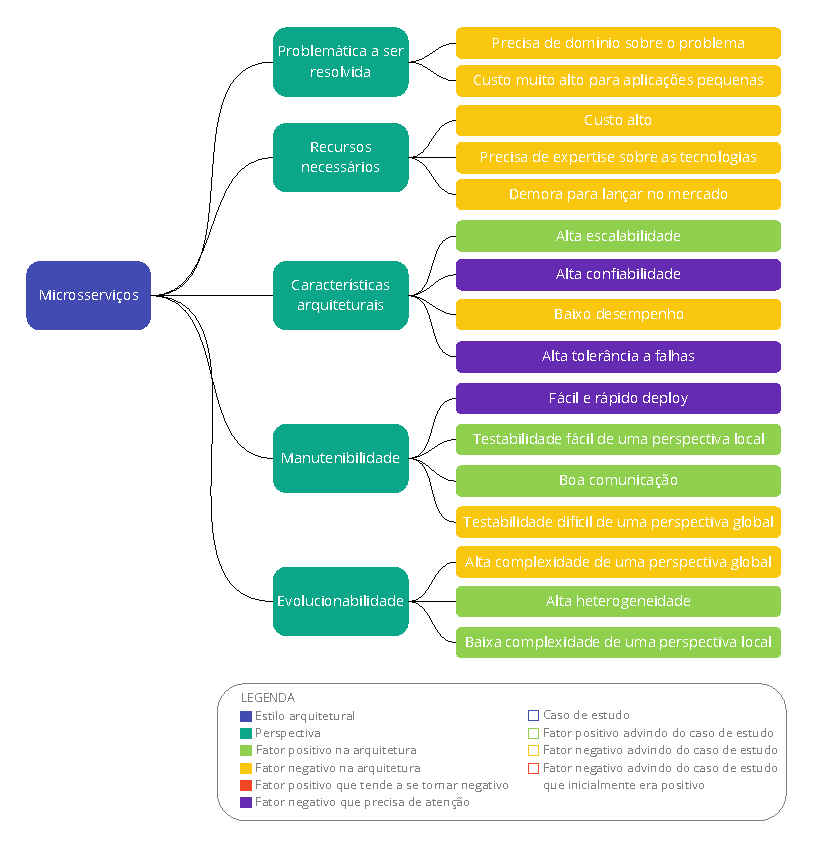
\includegraphics[keepaspectratio=true,scale=1]{figuras/sintese-microsservicos.eps}
  \caption{Mapa mental do processo de síntese realizado sobre a arquitetura de microsserviços\label{fig:SinteseMicro}}
\end{figure}


\newpage

        % \begin{description}
        %     \item [Problemática a ser resolvida:] perspectiva a respeito do contexto inicial da
        %         aplicação;
        %     \item [Recursos necessários:] perspectiva a respeito dos recursos financeiros, humanos,
        %         esforços e de tempo necessários para cada arquitetura;
        %     \item [Características arquiteturais:] capacidade da arquitetura de prover
        %         escalabilidade, tolerância a falhas, etc.
        %     \item [Manutenibilidade:] visão a respeito de processos cotidianos relacionados a
        %         manutenção do sistema;
        %     \item [Evolucinabilidade:] visão a respeito das características arquiteturais que
        %         influênciam na evolução do sistema.
        % \end{description}
%
% \begin{itemize}
%     \item Problemática da aplicação
%         \begin{itemize}
%             \item Domínio do contexto
%             \item Tamanho da aplicação
%         \end{itemize}
%     \item Recursos
%         \begin{itemize}
%             \item Recursos financeiros
%             \item Recursos humanos
%             \item Esforço inicial e tempo
%         \end{itemize}
%     \item Características arquiteturais 
%         \begin{itemize}
%             \item Escalabilidade
%             \item Tolerância a falhas
%             \item Confiabilidade
%             \item Performance
%         \end{itemize}
%     \item Manutenibilidade
%         \begin{itemize}
%             \item \textit{Deploy}
%             \item Testabilidade
%             \item \textit{Debugger}
%             \item Comunicação
%         \end{itemize}
%     \item Evolucionabilidade 
%         \begin{itemize}
%             \item Heterogeneidade das tecnologias
%             \item Complexidade
%         \end{itemize}
% \end{itemize}

\section{Análise dos casos de estudo}

A presente seção visa relatar casos reais de empresas que vivenciaram os estilos arquiteturais
estudados. A proposta é entender o contexto dessas empresas, as decisões tomadas e qual a percepção
que elas obtiveram sobre seus sistemas ao experimentar diferentes arquiteturas.

Serão abordados três casos:

\begin{enumerate}
    \item \textbf{KN Login:} um monolítico legado transformado em uma série de sistemas
        autocontidos, com o intuito de caminhar em direção a uma arquitetura de microsserviços;
    \item \textbf{Otto:} a reimplementação do zero de um monolítico em uma arquitetura de sistemas
        autocontidos que posteriormente é evoluída para microsserviços;
    \item \textbf{Segment}: a transição de um monolítico para uma arquitetura de microsserviços,
        seguido do retorno para a arquitetura monolítica após as várias dificuldades encontradas.
\end{enumerate}

\subsection{KN Login}
\label{sec:KNLogin}

O caso apresentado nessa seção é um relato de \citeonline{Olga2016:SelfContainedSystems} a respeito
da transição realizada por Björn Kimminich\footnote{Gerente sênior de arquitetura de TI na empresa
Kuehne + Nagel. Mais informações em: \url{https://www.linkedin.com/in/bkimminich}} e sua equipe na empresa
Kuehne + Nagel\footnote{Vide \url{https://home.kuehne-nagel.com}} de um sistema monolítico para sistemas
auto-contidos\footnote{O relato original e completo da autora sobre o caso pode ser encontrado no link
\url{https://www.elastic.io/breaking-down-monolith-microservices-and-self-contained-systems/}}. 

A Kuehne + Nagel é uma empresa especializada em transportes e logística que presta serviços em uma
escala global. Dentre as aplicações de software utilizadas na empresa para entrega dos seus
produtos, existe um serviço chamado KN Login, o qual proporciona diversas funcionalidades
importantes para a empresa, como gerenciamento dos contêineres transportados, auxilia no controle da
integridade e eficiência da cadeia de suprimentos de seus clientes, rastreio dos contêineres com
análise das condições ambientais, etc.

\subsubsection{Problemática da aplicação}

O KN Login é um sistema monolítico iniciado em 2007 construído em cima do \textit{framework}
Java Web\footnote{Vide \url{https://docs.oracle.com/javase/7/docs/technotes/guides/javaws/developersguide/overview.html}}.
Inicialmente foi construído como uma aplicação simples mas com o passar do tempo se tornou um imenso
monolítico com mais de um milhão de linhas de código e com uma grande variedade de atribuições e
responsabilidades dentro da empresa. Esse contexto trouxe a equipe de software da Kuehne + Nagel as
seguintes dificuldades:

\begin{itemize}
    \item A impossibilidade de trocar o \textit{framework} Java Web para outra tecnologia que se
        adeque melhor as necessidades da empresa, uma vez que o \textit{framework} se encontra enraizado no sistema;
    \item A manutenção de dois \textit{frameworks} em paralelo na mesma aplicação, visto que, a
    equipe de \gls{TI} deles recomenda o uso do Spring Framework\footnote{Vide \url{https://spring.io}} em
    detrimento do Java Web Framework sempre que possível;
    \item Várias tecnologias diferentes de \gls{UI} utilizadas para conseguir atender as diferentes
    problemáticas enfrentadas pela empresa;
    \item O sistema se tornou bastante instável mediante a vasta variedade de tecnologias aplicadas,
    tornando difícil a manutenção do mesmo pela equipe;
    \item Alta complexidade que dificulta a entrada de novos membros no time de desenvolvimento.
\end{itemize}

\subsubsection{Solução adotada}

Mediante as dificuldades enfrentadas, a Kuehne + Nagel optou por seguir os seguintes passos:

\begin{itemize}
    \item Parar de adicionar quaisquer funcionalidades ou modificações no sistema por mais
        importante que estas sejam para o escopo do negócio;
    \item Identificar os módulos e limites do monolítico, de forma que fosse possível criar uma
        separação ou até mesmo cortar tais partes do monolítico;
    \item Ter ciência de quão dependentes são cada módulo dentro do monolítico, de tal forma que
        alguns sejam aparentemente impossíveis de separar;
    \item Começar a separação de cada módulo aos poucos, de maneira que pedaços possam ser
        desativados no monolítico a medida que cada novo módulo é liberado;
\end{itemize}

Após analisar esses quatro fatores, a equipe técnica da Kuehne + Nagel chegou ao ponto de que a
mudança diretamente para microsserviços seria inviável mediante a grande complexidade do monolítico,
além de que esta mudança não iria contribuir para deixar mais fácil a visualização que eles
tinham do sistema. Diante desta situação a equipe optou por abordar uma arquitetura de sistemas
autocontidos\footnote{Abordagem arquitetural que consiste em quebrar o sistema em vários sistemas
independentes, cada um com sua propría \gls{UI}, camada de lógica e persistência de dados.}.

Sistemas autocontidos segundo \citeonline{Olga2016:SelfContainedSystems}, diference dos
microsserviços por serem aplicações web autônomas e substituíveis as quais tendem a ser maiores do
que um microsserviço e possuem uma unidade de \gls{UI} própria. Assim, a Kuehne + Nagel construiu o
seu primeiro sistema autocontido chamado KN Freightnet, o qual contou com a duplicação de algumas
funcionalidades presentes no KN Login, representando o primeiro passo para minimizar a complexidade
do KN Login.

\subsubsection{Panorama pós-adoção da solução}

O relato apresentado por \citeonline{Olga2016:SelfContainedSystems}, não traz informações a respeito
de quais foram os resultados efetivos da adoção de sistemas autocontidos mediante as dificuldades
que a equipe enfrentava dentro no monolítico KN Login, mas a autora traz a perspectiva de utilizar
sistemas autocontidos como um passo intermediário em direção aos microsserviços quando o monolítico
em mãos tem uma complexidade muito alta para ser quebrado.

\subsubsection{Análise sobre o caso de estudo}

O caso da KN Login traz a típica história dos monolíticos: inicialmente uma aplicação que deveria
ser simples mas que com o tempo o sistema foi inflando com várias funcionalidades. Nota-se que a
equipe do KN Login se deparou com um contexto complexo: rastreio dos contêineres, análise climática,
etc. E mediante esse contexto, eles tentaram lidar com toda a problemática dentro do monolítico sem
considerar a limitação que este estilo arquitetural oferece referente a heterogeneidade das
tecnologias envolvidas.

Diante da combinação: contexto complexo e heterogeneidade de tecnologias, o monolítico KN Login
resultou em uma aplicação de alta complexidade e baixa confiabilidade, se tornando um sistema
instável e difícil de manter. A \autoref{fig:monoKN} visa ilustrar os pontos destacados na
arquitetura monolítica do KN Login mediante aos fatores levantados sobre essa arquitetura na
\autoref{monoSintese}. 

\begin{figure}[h]
  \centering
  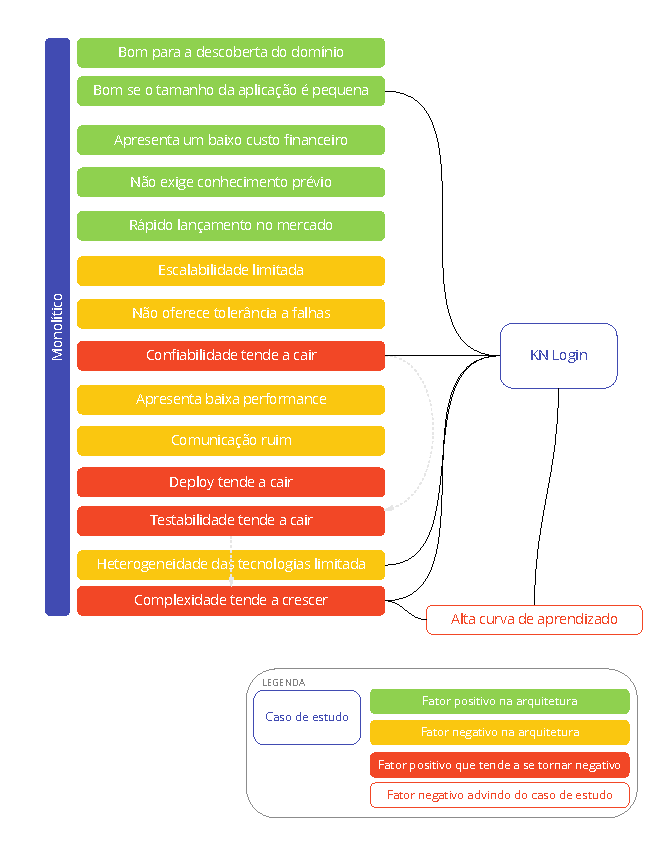
\includegraphics[keepaspectratio=true,scale=1]{figuras/analise-knlogin.eps}
  \caption{Fatores apresentados no caso de estudo da arquitetura monolítica do sistema KN Login\label{fig:monoKN}}
\end{figure}

\subsection{Otto}

Nesta seção será apresentado o caso relatado por  \citeonline{Guido2015:OnMonolithsAndMicrosrvices}, a
respeito da construção do novo \textit{e-commerce} Otto\footnote{O relato original e completo do autor
sobre o caso pode ser encontrado nos links
\url{https://www.otto.de/jobs/technology/techblog/artikel/on-monoliths-and-microservices_2015-09-30.php}
e \url{https://www.otto.de/jobs/technology/techblog/artikel/why-microservices_2016-03-20.php}}.O Grupo
Otto\footnote{Vide: \url{https://www.otto.de}} é uma empresa de origem alemã que trabalha em diversos países
desenvolvendo soluções de negócios voltadas a necessidade do setor de \textit{e-commerce}.

\subsubsection{Problemática da aplicação}

O sistema da Otto originou-se inicialmente em um projeto que deveria ser simples, no qual
implicitamente a equipe adotou uma macroarquitetura monolítica sem considerar ou até mesmo enxergar
que tal decisão estava sendo tomada. E mediante tal decisão, a equipe passou a ter dificuldades
com os problemas apresentados abaixo:

\begin{itemize}
    \item Escalabilidade limitada ao balanceamento de carga;
    \item Dificuldade de manutenção crescia juntamente com o crescimento da aplicação;
    \item Dificuldade de contratar desenvolvedores dispostos a trabalhar em um sistema de alta
        complexidade;
    \item Dificuldades ao realizar o \textit{deploy} principalmente no caso de aplicações sem
        períodos de inatividade;
    \item Dificuldades para trabalhar com várias equipes diferentes em uma mesma aplicação.
\end{itemize}

\citeonline{Guido2015:OnMonolithsAndMicrosrvices} enfatiza três pontos que para ele são importantes:

\begin{itemize}
    \item O desenvolvimento começa em equipe e no início a aplicação é bastante compreensível,
        necessitando apenas de uma única aplicação;
    \item Quando se tem um único aplicativo, o custo inicial é relativamente baixo: construção do
        repositório, automatização da \textit{build} e do processo de \textit{deploy}, configurar
        ferramentas de monitoramento, etc. Ativar e operar um novo aplicativo é relativamente fácil;
    \item É mais complexo operar grandes sistemas distribuídos do que um \textit{cluster}
        balanceador de carga.
\end{itemize}

\subsubsection{Solução adotada}

Diante do contexto apresentado, a Otto decidiu por começar um novo sistema de \textit{e-commerce},
adotando dessa vez uma arquitetura semelhante a apresentada na \autoref{sec:KNLogin} de sistemas autocontidos. Para
tal, eles estabeleceram quatro equipes funcionais dando origem a quatro aplicações. Os custos
iniciais de cada aplicação foram minimizados padronizando o processo de automação.

A medida que o sistema da Otto evoluía foram criados novos sistemas autocontidos, cada um com sua própria equipe
de desenvolvimento, seu próprio \textit{frontend} e seu próprio
banco de dados, tudo dentro de um escopo de negócio muito bem definido a respeito das suas
atribuições.

A Otto definiu aspectos macro e microarquiteturais. Os aspectos
microarquiteturais estavam voltados ao contexto local de cada sistema autocontido construído,
enquanto que nos aspectos macro foram definidos questões mais globais a respeito da arquitetura, como por exemplo:

\begin{itemize}
    \item A comunicação entre os sistemas autocotidos deveria ser feita sempre por meio do modelo
        \gls{REST};
    \item Não poderia existir estado mutável compartilhado entre as aplicações;
    \item Os dados devem ser compartilhados por meio de uma \gls{API} \gls{REST}, havendo somente
        uma aplicação responsável pelo dado e as outras unicamente com a permissão de leitura sobre o
        mesmo.
\end{itemize}

Nessa abordagem arquitetural escolhida, a Otto se deparou com dificuldades no compartilhamento
de dados entre as aplicações, o que os levou a adotar a estratégia de replicação de dados, na qual,
eventualmente eles precisam lhe dar com inconsistências temporárias entre os sistemas.

Contudo, alguns sistemas autocontidos ficaram bastante volumosos após cerca de três anos trabalhando
em cima dessa arquitetura. Essa nova situação fez com que a Otto adota-se uma nova medida em direção
a uma arquitetura de microsserviços. Decisão esta que segundo \citeonline{Guido2016:WhyMicroservices}
não gerou um processo tão árduo dentro da empresa uma vez que eles já vinham trabalhando em cima de
uma arquitetura bastante modularizada e já trabalhavam de forma concisa as questões de limites de
cada aplicação.

\subsubsection{Panorama pós-adoção da solução}

Após a adoção de uma arquitetura autocontida e a migração para uma arquitetura de microsserviços,
\citeonline{Guido2016:WhyMicroservices} traz como pontos positivos de ambas as arquiteturas os
seguintes pontos:

\begin{itemize}
    \item Facilidade em estabelecer uma pirâmide de testes que funcione de forma eficiente e rápida,
        auxiliando os desenvolvedores no lançamento de novas versões do código;
    \item Facilidade em gerenciar e integrar o trabalho de diferentes equipes uma vez que cada uma
        está trabalhando em seu próprio serviço;
    \item Aumento na velocidade de implantação de novas funcionalidades, sendo mais fácil testar e
        coletar rapidamente \textit{feedback};
    \item Cada aplicativo pode ser implementado de forma independente;
    \item Não há necessidade de coordenar o processo de implantação, cada equipe possui autonomia
        para gerenciar o seu processo de implantação sem afetar as demais equipes;
    \item Baixa curva de aprendizado, cada serviço é de fácil compreensão pelos desenvolvedores;
    \item Escalabilidade em relação a aplicação e aos próprios times de desenvolvimento;
    \item A complexidade de um serviço é extremamente baixa quando comparada a uma arquitetura
        monolítica;
    \item O sistema não está limitado a uma tecnologia específica;
    \item Exige que todos os processo estejam automatizados;
    \item Facilidade em reverter a versão do projeto quando algum \textit{bug} é introduzido;
    \item A ocorrência de falhas não afeta o sistema por inteiro, somente uma parte dele;
    \item Permite manter com facilidade a alta coesão e o baixo acoplamento do sistema;
\end{itemize}

Segundo a visão do autor, os microserviços possibilitam a construção de um sistema de software muito
mais sustentável ao longo dos anos do que um sistema monolítico, de forma que nessa arquitetura é
possível substituir pequenos pedaços da aplicação quando for necessário, enquanto que em sistemas
monolíticos essa abordagem se torna muito mais complexa.

A adoção de sistemas autocontidos é apresentada por ele como uma porta de entrada na qual é possível
resolver problemas semelhante aos microsserviços de uma forma mais pragmática, deixando ainda a
possibilidade de migrar futuramente para uma arquitetura de microsserviços de uma forma não tão
árdua \cite{Guido2016:WhyMicroservices}.
    
\subsubsection{Análise sobre o caso de estudo}

A figura \autoref{fig:analise-mono-otto} ilustra os pontos da arquitetura monolítica levantados pelo
caso de estudo da Otto. Percebe-se que a experiência deles atesta os pontos referentes ao início do
projeto quando a aplicação é pequena, de fácil compreensão por todos, tem um custo baixo, etc.
Também atesta os problemas de complexidade e de implantação que tendem nesse modelo arquitetural a
crescer juntamente com a base de código.


\begin{figure}[h]
  \centering
  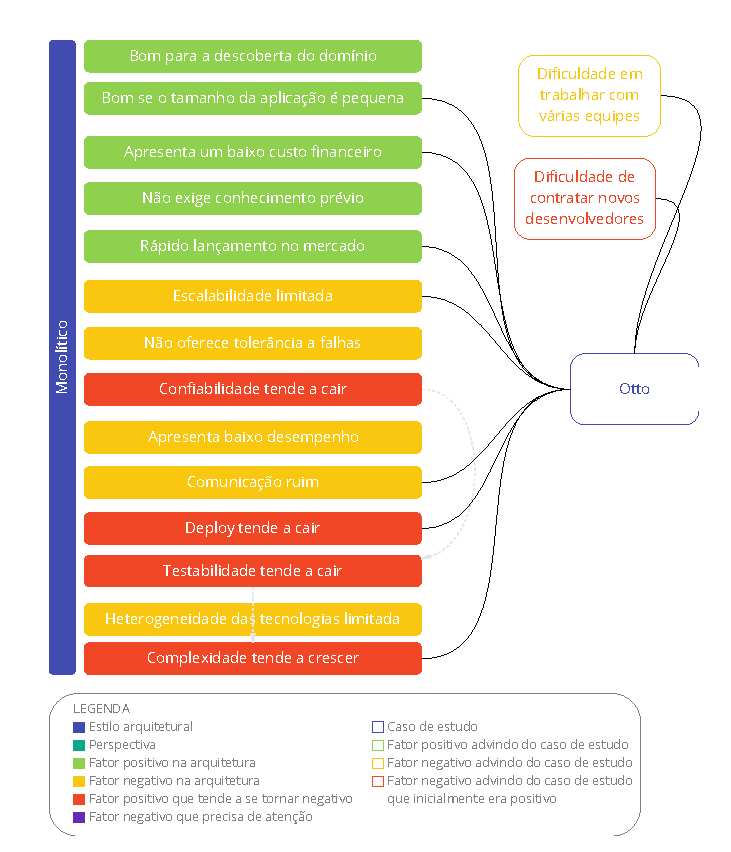
\includegraphics[keepaspectratio=true,scale=1]{figuras/monoOtto.eps}
  \caption{Fatores apresentados no caso de estudo da arquitetura monolítica da Otto\label{fig:analise-mono-otto}}
\end{figure}

A tomada de decisão por migrar para uma arquitetura de sistemas auto-contidos auxilia eles como um
passo intermediário antes de aderir toda a complexidade da arquitetura de microsserviços. Nessa
abordagem percebe-se que eles vivenciam características dos dois estilos arquiteturais. Olhando da
perspectiva dos microsserviços, eles definem protocolos de comunicação e compartilhamento de dados e lidam
com eventuais inconsistência de dados (um problema comum da arquitetura de microsserviços). Por
outro lado, eles ainda precisam lidar com a crescente base de código dos monolíticos dentro de cada
sistema auto-contido.

A figura \autoref{fig:analise-micro-otto} ressalta os pontos da arquitetura de microsserviços
adotada pela Otto, na qual nota-se alta escalabilidade, alta tolerância a falhas, facilidade no
\textit{deploy}, testabilidade e alta heterogeneidade de tecnologias observados no caso de estudo.
A experiência da Otto também traz outros pontos dessa arquitetura, não presentes no mapa mental
construído, como baixa curva de aprendizado e a necessidade de automatizar todos os processos.  

Um ponto que se diferencia do esperado, de acordo com a fundamentação teórica levantada para esse
trabalho, é que a Otto apresenta a coleta de \textit{feedbacks} como um ponto positivo da
arquitetura de microsserviços enquanto o referencial teórico aponta a arquitetura monolítica como
mais indicada para tal. Nesse sentido, percebe-se que existe o fator tempo de projeto envolvido.
Como relatado na \autoref{Perspectivas:Problematica} e na \autoref{effortsAndTime}, ao iniciar um
projeto a arquitetura monolítica é melhor para a rápida coleta de \textit{feedbacks} por ser mais
simplista, contudo no caso da Otto, eles já tinham um sistema monolítico com uma base de código
grande e devido aos problemas de complexidade já discutidos evoluir e testar rápido esse sistema com
os usuários já não deveria ser um processo tão fácil. Já na arquitetura de microsserviços, existe o
esforço inicial de automatizar todos os processos e de planejar cuidadosamente os limites de domínio
de cada aplicação, mas após essas etapas estarem bem definidas alterar e testar novos serviços tende
a ser fácil.

\begin{figure}[h]
  \centering
  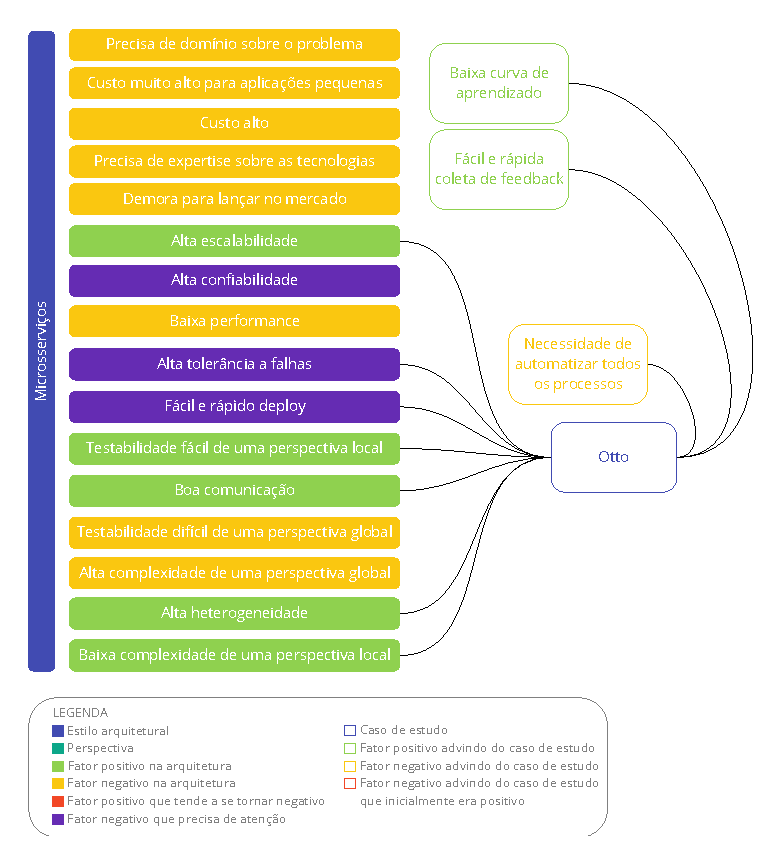
\includegraphics[keepaspectratio=true,scale=1]{figuras/analise-micro-otto.eps}
  \caption{Fatores apresentados no caso de estudo da arquitetura de microsserviços da Otto\label{fig:analise-micro-otto}}
\end{figure}

\subsection{Segment}

O caso apresentado a seguir foi retratado por \citeonline{Noonan:ToMicroservicesAndBackAgain} na
conferência QCon London. Ela trata a respeito do sistema da Segment\footnote{Vide:
\url{https://segment.com}}, o qual foi construído inicialmente em uma arquitetura monolítica,
passou por uma migração para uma arquitetura de microsserviços e após 3 anos em cima desta
arquitetura, decidiram por retornar para a arquitetura monolítica.

A Segment é uma empresa responsável por fazer a integração entre as aplicações de software de seus
clientes com diversas ferramentas de análise de dados, atuando como um \textit{pipeline} facilitador
na integração entre as partes citadas. 

\subsubsection{Problemática da aplicação}

Em 2013, quando a empresa foi criada havia necessidade de construir um sistema que possuísse uma
baixa sobrecarga operacional, sendo simples de gerenciar e fácil de iterar, assim, diante de tais
necessidades a primeira versão do sistema da Segment foi construído em cima de uma arquitetura monolítica.

A arquitetura inicial consistia em uma \gls{API} de entrada que recebia os dados enviados pelas aplicações dos
clientes da Segment, e colocava esses dados em uma fila de processamento. A partir deste ponto,
havia uma monolítico responsável por consumir a fila e enviar os dados para as aplicações de destino
(Google Analytics, Salesforce...). O consumo dessa fila ocorria no modelo \gls{FIFO}\footnote{Vide
\url{https://pt.wikipedia.org/wiki/FIFO}}. A dificuldade enfrentada pela equipe da Segment nessa
arquitetura estava na tentativa de reenviar algum dado quando por algum motivo a primeira tentativa
tinha falhado. De acordo com \citeonline{Noonan:ToMicroservicesAndBackAgain}, cerca de 10\% das
solicitações para as aplicações de destino falhavam e nesses casos, o monolítico fazia de 2 a 10
tentativas de reenvio.

Nessa abordagem, a Segment passou a enfrentar um bloqueio frontal na fila. Sempre que uma aplicação
de destino estava muito instável ou ficava fora do ar, o monolítico travava a fila tentando refazer
o envio, de forma que o problema se propagava: ao invés de ter uma integração X fora do ar, todas as
outras integrações também paravam de funcionar visto que a fila estava bloqueada.

Após um ano trabalhando em cima dessa arquitetura, o time de desenvolvimento da Segment decidiu por
mudar para uma arquitetura de microsserviços visando o isolamento do ambiente, de forma que
problemas com uma determinada integração não impactasse na outra. Para tal, eles segregaram cada
integração em um serviço próprio acompanhado de sua própria fila e adicionaram antes das filas um
roteador capaz de receber os dados da \gls{API} de entrada e direcioná-los para as filas necessárias.
Essa abordagem trouxe as seguintes vantagens para a Segment:

\begin{itemize}
    \item Diminui a necessidade de \textit{backup} da fila, uma vez que ao falhar uma aplicação de
        destino eles não precisam mais salvar a fila toda, mas somente a parte referente a
        integração problemática;
    \item A falha em uma aplicação de destino não afetava mais as outras integrações;
    \item Facilitou a inserção de novas aplicações de destino ao sistema da empresa, permitindo um
        desenvolvimento mais rápido;
    \item Facilidade em tratar as peculiaridades de cada integração dentro do seu próprio serviço,
        sem precisar compatibilizar os dados com todas as aplicações de uma única vez;
    \item Agregou a visibilidade de toda a pilha do processo, permitindo identificar mais facilmente
        as falhas e a qual serviço específico elas eram referentes.
\end{itemize}

Em 2016, a Segment possui 50 serviços integrando diferentes aplicações. Com o aumento na quantidade
de serviços para gerenciar eles começaram a ter algumas dificuldades, entre elas:

\begin{itemize}
    \item Não possuíam processos de \textit{build} e \textit{deploy} automatizados, o que acaba
        exigindo bastante tempo da equipe mediante a quantidade de serviços no ar;
    \item Cada sistema realizava diferentes tratamentos sobre o dado antes de enviar para a
        aplicação de destino e como cada cliente podia enviar os dados de diferentes formas, acabou
        se tornando árduo entender o que estava se passando dentro de cada serviço. Nesse caso, eles
        optaram por criar bibliotecas comuns entre os serviços para fazer tal tratamento.
        Inicialmente, isto se refletiu positivamente dentro da equipe, mas sem os processos de
        implantação automatizados, a atualização da versão das bibliotecas em cada serviço se tornou
        um problema de tal forma que eles passaram a preferir não corrigir um \textit{bug} dentro da
        biblioteca do que fazer a atualização;
    \item Administrar o escalonamento da arquitetura não era uma tarefa fácil. Alguns clientes
        geravam um tráfego de milhares de requisições por segundo, e frequentemente acontecia de
        algum desses clientes ativarem alguma integração com o intuito de experimentar, e apesar das regras
        automáticas de escalonamento e dimensionamento de recursos, o time de \gls{TI} da Segment
        não conseguia encontrar uma regra de escalabilidade que se adequasse bem ao contexto deles.
        Diante desse caso, eles pensaram em soluções de supervisionamento da arquitetura, manter
        sempre alguns trabalhadores mínimos, etc., mas chegaram a conclusão de que essas abordagens
        teriam um custo muito alto para a empresa;
    \item Mesmo com todas as dificuldades, eles continuavam adicionando cerca de três aplicações de
        destino por mês. O que tornava cada vez mais complexa a base de código e fazia a carga
        operacional, diante dos processos não automatizados, crescer linearmente ainda que o tamanho
        da equipe fosse constante;
    \item A empresa chegou a parar de desenvolver novas funcionalidades visto que a complexidade e a
        dificuldade para manter os microsserviços funcionando estava altíssima;
    \item A carga encaminhada dos clientes havia aumentado consideravelmente e eles ainda
        continuavam com o mesmo problema de limitação do tráfego pelo lado das aplicações de
        destino, o mesmo bloqueio frontal mencionado anteriormente;
\end{itemize}

\subsubsection{Solução adotada}

Em 2017, \citeonline{Noonan:ToMicroservicesAndBackAgain} relata que eles chegaram ao ponto de
ruptura: haviam 140 serviços rodando, uma equipe pequena mantendo uma série de processos
operacionais e uma base de código complexa fazendo com que a arquitetura que inicialmente parecia
ideal e que os auxiliaria a escalar, se torna-se o fator paralisador de todo o sistema. Nesse ponto,
eles reunirão todas as experiências que haviam reunido desde 2013, e tomaram a decisão de retornar
para uma arquitetura monolítica, com um sistema único que eles fossem capaz de gerenciar e escalar.

A solução adotada reuniu todas as 140 integrações no mesmo repositório novamente, ao invés de ter
uma fila para cada aplicação eles optaram por salvar os dados em um banco MySQL\footnote{Vide
\url{https://www.mysql.com}}, com as condições de que:

\begin{itemize}
    \item As linhas do banco deveriam ser imutáveis, devendo o monolítico sempre inserir o novo
        estado mas nunca atualizar o antigo;
    \item Operações de JOIN não deveriam ser realizadas. No modelo desenvolvido por eles, o
        monolítico deveria apenas ler informações básicas sobre os dados a serem tratados;
    \item A escrita deve ser a operação predominante. Nessa nova arquitetura, a maioria dos dados
        eram tratados em cache e tinham apenas o seu estado registrado no banco de dados.
\end{itemize}

Dessa forma, os dados chegavam ao monolítico, o qual registrava os mesmos no banco mas ainda os
mantinham em cache. A medida que os dados eram tratados, o monolítico removia os dados do cache e
registrava o novo estado no banco. Quando alguma integração falhava, o estado de falha era
registrado no banco para que fosse tratado posteriormente por meio da estratégia de \textit{backoff}
definida por eles.

Olhando a perspectiva da escalabilidade, o monolítico podia ser replicado sempre que houvesse a
necessidade. Para tal, havia um serviço responsável por gerenciar as instâncias de banco de dados.
Sempre que um novo monolítico era colocado no ar, ele recebia por meio desse serviço o acesso a um
banco de dados exclusivamente seu. Dessa forma, eles conseguiram automatizar o processo de
escalabilidade de acordo com o uso da CPU \cite{Segment2018:Centrifuge}\footnote{A descrição
completa da solução adotada pela Segment pode ser encontrada no link \url{https://segment.com/blog/introducing-centrifuge/}}.

\subsubsection{Panorama pós-adoção da solução}

A solução adotada pela Segment permitiu a eles:

\begin{itemize}
    \item Escalar melhor a sua aplicação, lidando de forma mais eficiente com as limitações de
        capacidade das aplicações destino e permitindo a adição de novos serviços sem a necessidade
        de aumentar os custos operacionais da equipe;
    \item Aumentou consideravelmente a produtividade do time;
    \item Solucionou o problema de compatibilidade de diferentes versões de bibliotecas
        compartilhadas entre os serviços;
    \item Facilitou o desenvolvimento de novas funcionalidades para o sistema;
\end{itemize}

Os problemas que eles tinham na primeira arquitetura monolítica relacionados às dificuldades de
isolamento de ambiente continuaram presentes nessa nova arquitetura, contudo, agora o time de
desenvolvimento da Segment soube lhe dar de forma muito mais madura com essa situação, procurando
outras soluções diferente de microsserviços para tratar os obstáculos com os quais eles se
deparavam.

\subsubsection{Análise sobre o caso de estudo}

O caso da Segment conta com três fases que precisam ser avaliadas: o monolítico inicial, os
microsserviços e o monolítico final. A figura \autoref{fig:analise-mono-segment-1} representa o
primeiro monolítico construído pela empresa. A escolha inicial de uma arquitetura monolítica condiz
com o contexto da empresa, a qual era composta por uma equipe pequena de engenheiros de software e
estava buscando validar sua ideia e descobrir o domínio no qual estavam imersos. 

\begin{figure}[h]
  \centering
  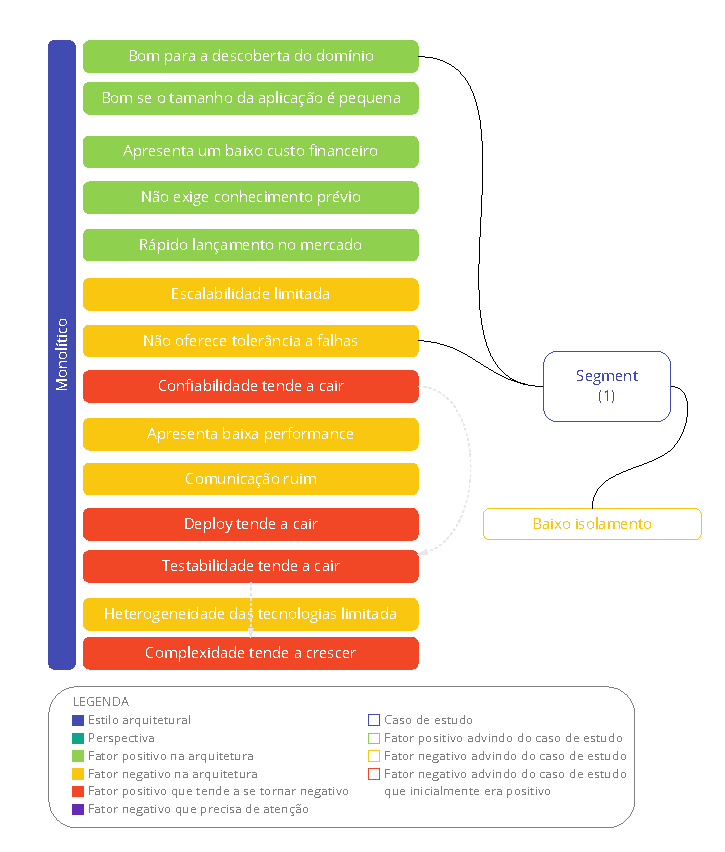
\includegraphics[keepaspectratio=true,scale=1]{figuras/analise-mono-segment-1.eps}
  \caption{Fatores apresentados no caso de estudo da primeira arquitetura monolítica da Segment\label{fig:analise-mono-segment-1}}
\end{figure}

No caso, a Segment se depara logo com a limitação de tolerância a falhas dessa arquitetura e decidem
mudar para uma arquitetura de microsserviços. Visto que o sistema da Segment era um software novo,
com um ano de funcionamento quando eles optaram por fazer a migração, percebe-se que outros problemas
da arquitetura monolítica não aparecem no relato, como alta complexidade, dificuldades de
manutenibilidade, etc., evidenciando o ponto levantado na \autoref{monoSintese} de que essas
características são inicialmente positivas no sistema e estão diretamente relacionadas ao tamanho da
base de código.

Ao passar o sistema para a arquitetura de microsserviços, o time consegue perceber os pontos
destacados na \autoref{fig:analise-micro-segment} como a tolerância a falhas, a baixa complexidade
local, etc. Vale ressaltar que a Segment também relata, semelhante a Otto, a facilidade e velocidade
de adicionar novas funcionalidades nessa arquitetura. Contudo, percebe-se também a ausência da expertise,
comentada na \autoref{Perspectivas:recursosHumanos}, sobre este modelo arquitetural visto que os processos
operacionais não são automatizados pela equipe da Segment. Este fator somado ao crescente número de
serviços funcionando faz com que a equipe se afogue na grande demanda de processos operacionais
exigida por essa arquitetura. Assim, eles param todo o desenvolvimento mediante a inviabilidade de
gerenciar essa arquitetura nas proporções que ela tomou.

\begin{figure}[h]
  \centering
  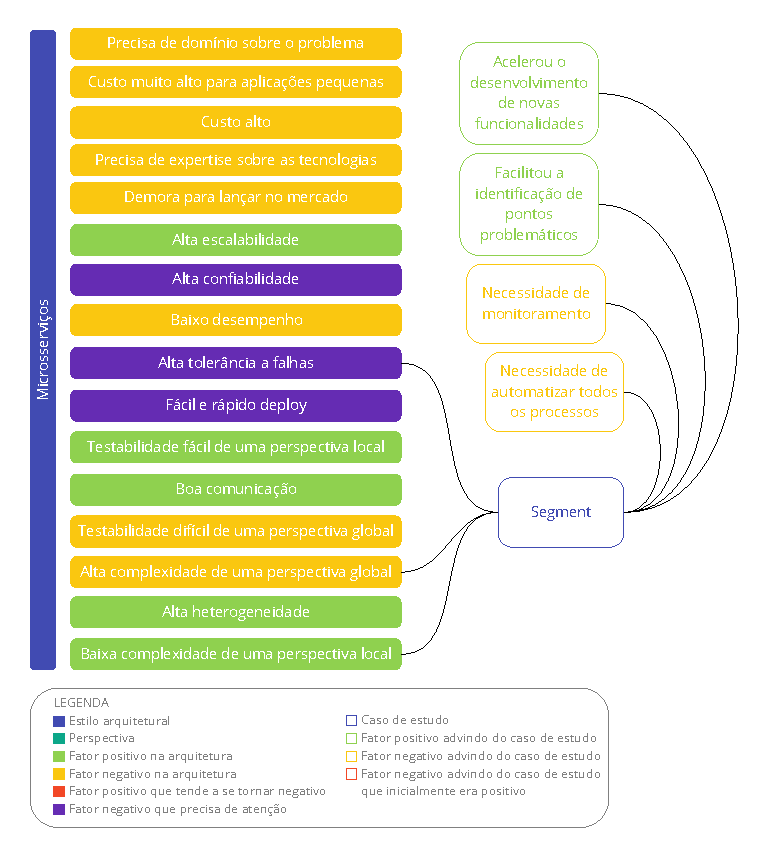
\includegraphics[keepaspectratio=true,scale=1]{figuras/analise-micro-segment.eps}
  \caption{Fatores apresentados no caso de estudo da arquitetura de microsserviços da Segment\label{fig:analise-micro-segment}}
\end{figure}

No meio desta situação, a Segment opta por voltar para a arquitetura monolítica mas de uma forma
mais consciente sobre quais eram as dificuldades do contexto deles, planejando estratégias para
lidar com as adversidades que eles já conheciam. Assim, eles conseguem construir um sistema que
possa prover escalabilidade, tolerância a falhas e produtividade para a equipe em cima de uma
arquitetura monolítica. Vale salientar que, a respeito da produtividade da equipe, a Segment se
encontra com um monolítico relativamente novo, que foi planejado e assim ele apresenta o perfil de
um monolítico em sua fase inicial: baixa complexidade, módulos bem definidos, etc., contudo, é
necessário que a equipe se empenhe para conseguir manter essas características a medida que sua base
de código cresce.

% Esta seção tem por propósito apresentar o estudo realizado sobre a
% \textit{startup} Rua Dois Tecnologias, sendo esta o objeto de análise
% central do presente trabalho. O escopo deste capítulo abrangerá desde
% o entendimento sobre o contexto da empresa e sua proposta de valor
% até aspectos mais técnicos como a arquitetura do sistema, sua evolução
% durante o primeiro ano da empresa e as dificuldades enfrentadas pela
% \textit{startup} nessa arquitetura.
%
%   As seções estão dispostas em:
%
%   \begin{enumerate}
%     \item \textbf{Rua Dois Tecnologias:} breve apresentação sobre a empresa,
%       seus propósitos e os serviços oferecidos;
%     \item \textbf{Arquitetura do sistema:} descrição da arquitetura de software
%       adotada dentro da Rua Dois, no seu primeiro ano de desenvolvimento, e possíveis
%       soluções discutidas dentro da empresa a respeito da escalabilidade.
%   \end{enumerate}
%
% \section{Rua Dois Tecnologias}
%
% No artigo \textit{Modernizing Real Estate: The Property Tech Opportunity}
% \footnote{Disponível
% \href{https://www.forbes.com/sites/valleyvoices/2019/02/22/the-proptech-opportunity}{nest link}.},
% a autora \citeonline{LouisaXu} aborda uma visão histórica sobre o desenvolvimento
% de tecnologias para o mercado imobiliário fazendo um comparativo com a realidade atual.
% Nesse histórico de desenvolvimento, ela relata que desde 1980 são empregados
% diversos esforços na área buscando melhorarias por meio de software, mas mesmo
% assim, continuamos em uma ramo altamente burocrático e carente de melhorias.
%
% Mediante essas limitações, surgiu em outubro de 2018 a Rua Dois Tecnologias,
% com o propósito de solucionar as dificuldades enfrentadas tanto por parte das
% imobiliárias quanto por parte dos locatários \footnote{Aquele que mora em um imóvel
% que não lhe pertence, mediante um contrato de locação.} no processo de locação de imóveis.
%
% A proposta\footnote{Mais informações a respeito da proposta e visão da Rua Dois podem
% ser encontradas
% \href{https://open.spotify.com/episode/2jYKPCPLCIdDWwxpR0theT?si=dT6WUG7JSEGJH3mVVIJitQ}
% {neste \textit{podcast}}.}
% da empresa consiste em atuar como um facilitador para as imobiliárias
% ingressarem no meio digital e consequentemente propiciar seu crescimento. Para tal,
% eles buscam aumentar a eficiência do processo de locação por meio da digitalização,
% proporcionando melhor integração entre operação e tecnologias. Assim, com um processo
% mais digital, os recursos humanos podem ser melhores empregados no atendimento do
% cliente favorencendo a experiência do mesmo nesse mercado tão burocrático.
%
%
% % Transformação Digital
% %     Inovação é criar valor
% %     Por meio de um processo mais digital entregar uma nova experiência para o usuário
% %     com mais eficiência e podendo se adaptar a novos modelos de negócio
% %     experiencia + eficiencia = novo modelo de negócio
% %     nova intereção do time
% %     digitalizacao markenting em vendas
% %     digitalização de produto
% %     liderança pela inovação
% %     fisico-digital
% %
% %     burocracia enorme
% %     perca de relacionamento com o cliente >> processo, automatizar, automatizar...
% %     voltar a um relacionamento muito grande mas com um alto grau de tecnologia envolvido nesse
% %     relacionamento entregando uma experiência melhor para o usuário e alcançando mais gente
% %
% %     dificuldade de crescer num mundo digital
% %
% %     proposito da rua dois: democratizar a experiência positiva de locação no brasil
% %     integração muito grande entre operação e tecnologia >> processos
% %     tecnologia + operação + serviço
% %     validação >> estatisticas >> crescimento da empresa
% %     lead >> direto para visita
%
% % TODO Conversar com o Erlan para melhorar essa parte
% % TODO Explicar o que é CEO e colocar nas lista de abreviações
% % TODO Descrever melhor o contexto e os papeis envolvidos
%
% \subsection{Serviços prestados}
%
% Visando o processo de locação de imóveis, a Rua Dois conta com quatro serviços
% sendo desenvolvidos dentro da empresa, afim de agregar valor aos seus clientes,
% sendo eles:
%
%   \begin{enumerate}
%     \item \textbf{Captação de Imóveis:} serviço destinado à atrair proprietários de
%       imóveis que desejam divulgar o imóvel para locação;
%     \item \textbf{Visitas:} serviço de visitas aos imóveis, no qual os interessados em
%       locar o imóvel agendam um horário para conhecer o mesmo;
%     \item \textbf{Propostas:} serviço no qual os interessados, após passarem pela etapa
%       de visitação, avaliam o imóvel e fazem uma proposta para o proprietário do
%       imóvel referente ao valor a ser pago pela locação e possíveis ajustes que
%       desejam que sejam feitos na propriedade;
%     \item \textbf{Contrato:} etapa final, destinada a automatizar a avaliação por parte
%       das seguradoras, envio de documentos e assinatura do contrato.
%   \end{enumerate}
%
% Cada serviço é vendido de forma separada para as imobiliárias, de forma que cada uma
% adapte ao seu contexto os serviços que melhor se encaixam. Atualmente, o serviço
% mais desenvolvido é o de visitas e a equipe vem trabalhando com o intuito de
% estabilizar os demais serviços.
%
% \section{Arquitetura do sistema}
% \label{sec:ArquiteturaDoSistema}
%
% O início do desenvolvimento do software da Rua Dois se deu em outubro de 2018 com
% base na proposta de criar um sistema usando de uma arquitetura de microsserviços, de
% forma que esse sistema já fosse preparado pra escalar desde seu início. Contudo,
% a empresa enfrentou uma série de dificuldades\footnote{Estas dificuldades serão abordadas
% com maior clareza na \autoref{sec:ArquiteturaFase1}} em relação a esta arquitetura e ao seu
% contexto no respectivo momento. Mediante essas dificuldades a Rua Dois optou em seu
% processo de desenvolvimento migrar essa arquitetura de microsserviços para um sistema
% monolítico.
%
% Esta seção visa descrever essas duas fases arquiteturais dentro da empresa com suas
% respectivas motivações e desafios encontrados. Assim, visando facilitar o entendimento,
% cada fase será nomeada da seguinte forma:
%
%     \begin{description}
%         \item [Fase 1] referente a fase inicial de desenvolvimento na qual foi adotada
%         uma arquitetura de microsserviços;
%         \item [Fase 2] referente a segunda fase de desenvolvimento na qual foi adotada
%         uma arquitetura monolítica.
%     \end{description}
%
%
% \subsection{Arquitetura do sistema: Fase 1}
% \label{sec:ArquiteturaFase1}
%
% A primeira fase de desenvolvimento da \textit{startup} foi marcada pela premissa de
% que o sistema deveria ser escalável, e com base nessa premissa foram tomadas uma
% série de decisões visando preparar o sistema para tal. Assim o sistema foi dividido 
% em dois microsserviços principais e em uma série de microsserviços auxiliares
% distribuídos nos lambdas da \gls{AWS}. Os dois serviços principais são:
%
%     \begin{description}
%         \item [r2service] responsável por gerir o cadastro de imóveis e as propostas
%         de locação do imóvel;
%         \item [r2visit] responsável por gerir a lógica de agendamento de visitas
%         a um imóvel.
%     \end{description}
%
% A \autoref{fig:ArquiteturaFase1} visa ilustrar a organização desse sistema. Nela
% os dois serviços principais estão representados pelos círculos maiores roxos e as
% demais representações são outros serviços que auxiliam no ciclo de vida do produto.
% Adiante segue descrito o fluxo com o qual todo o sistema é acionado, seguindo a
% enumeração disposta na imagem:
%
% \begin{figure}[h]
%   \centering
%   \includegraphics[keepaspectratio=true,scale=0.4]{figuras/r2ArquiteturaFase1.eps}
%   \caption{Arquitetura do sistema da Rua Dois na Fase 1\label{fig:ArquiteturaFase1}}
% \end{figure}
%
%   \begin{enumerate}
%     \item O \textit{Widget} é um componente utilizado pela Rua Dois que roda
%       no \textit{frontend} dos sites das imobiliárias que aderem ao serviço
%       de visitas. Ele se comunica com um lambda responsável por verificar se
%       o imóvel apresentado no site da imobiliária está disponível no banco
%       de dados da Rua Dois. Uma vez que esteja disponível, o \textit{widget}
%       exibe um botão que disponibiliza o agendamento da visita \textit{online}
%       para o interessado;
%     \item O locatário ao clicar nesse botão, dispara uma requisição ao lambda
%     que identifica o time de corretores responsável por atender as visitas
%     ao imóvel selecionado. E em seguida, uma nova requisição é disparada ao
%     serviço \textit{r2visit} solicitando o calendário com os horários
%     disponíveis do respectivo time;
%     \item Após o locatário ter selecionado o horário da visita, uma nova
%     requisição é lançada para registrar a visita no \textit{r2visit}, que por
%     sua vez dispara uma série de mensagens por meio das ferramentas de comunicação
%     e atualiza o Pipedrive\footnote{O Pipedrive é uma ferramenta de \gls{CRM} utilizada pela
%     empresa para realizar o gerenciamento operacional e monitoramento dos resultados obtidos.
%     Saiba mais em: \url{https://www.pipedrive.com}};
%     \item Após a visita ser realizada, o corretor sinaliza por meio do aplicativo
%     a conclusão da visita, disparando novamente no \textit{r2visit} os eventos
%     de atualização do Pipedrive e as ferramentas de comunicação, para que se
%     possa dar início a nova fase de Negociação, referente ao produto de propostas;
%     \item Nessa nova fase, locatário e locador trocam mensagens por meio do portal
%     da Rua Dois, o qual é gerido pelo \textit{r2service}. Ao final da negociação,
%     os clientes entram na fase de contrato, na qual seu dados são recolhidos e
%     enviados por meio do \textit{r2service} para \glspl{API} externas de seguradoras as quais
%     realizam uma avaliação de crédito do locatário. Quando concedida a avaliação
%     de crédito, o contrato é gerado automaticamente com os dados já recolhidos
%     do locatário, locador, da imobiliária e do próprio imóvel;
%     \item Por fim, o \textit{r2service} é responsável por atualizar uma planilha do
%     Google Sheets\footnote{Saiba mais em: \url{https://www.google.com/sheets/about/}}
%     que serve de insumo para geração de relatórios dentro do Data Studio
%     \footnote{Saiba mais em: \url{https://datastudio.google.com}}.
%   \end{enumerate}
%
% Nesse fluxo nota-se que existe uma grande diversidade de elementos interagindo entre
% si e a forma como isto foi organizado gerou as seguintes dificuldades dentro da empresa:
%
%     \begin{enumerate}
%         \item{Dificuldade de organização dos dados da empresa uma vez que não houve
%         um bom planejamento em relação a interação entre os serviços \textit{r2service}
%         e \textit{r2visit}, o que ocasionou a duplicação da tabela referente aos dados
%         dos imóveis - uma tabela no banco de dados da Virgínia e a outra tabela no banco
%         de dados de São Paulo;}
%         \item{Dificuldade de gerir as associações necessárias entre os dados armazenados
%         no banco. A empresa optou pelo uso do banco não relacional DynamoDB, visando
%         novamente a escalabilidade, mas sem planejar corretamente o armazenamento desses
%         dados nessa estrutura não relacional. Isso impactou diretamente o desenvolvimento,
%         visto que existe uma necessidade da empresa de tratar esse dado como relacional
%         mas fez isso em cima de uma tecnologia inadequada para tal;}
%         \item{Dificuldade de manter essa infraestrutura, tanto pela complexidade na forma
%         como o sistema está organizado quanto pela escolha de utilizar a infraestrutura da
%         \gls{AWS}, que é mais árdua de trabalhar do que outras soluções disponíveis no mercado
%         \cite{kavya};}
%         \item{Dificuldade de inserção de novos membros na equipe de desenvolvimento, visto
%         que entender como esses vários serviços se relacionam não é uma tarefa simples;}
%         \item{Dificuldade de mudança e inserção de novas funcionalidades. Nessa primeira
%         fase a Rua Dois encontrava-se fortemente no período de validação da ideia dentro
%         de uma \textit{startup} o que exigia uma rápida reação da equipe em relação aos
%         \textit{feedbacks} recebidos. Contudo, nessa arquitetura se tornou exaustivo a
%         realização de constantes mudanças vistos todos os problemas relatados nos tópicos
%         anteriores.}
%     \end{enumerate}
%
% % Desde seu início, a Rua Dois tem em seu modelo de negócio uma constante
% % preocupação com a escalabilidade do sistema. A empresa tem em seus objetivos
% % validar rapidamente a ideia e expandir para diferentes mercados. Contudo,
% % este objetivo foi alinhado a uma equipe de desenvolvimento de software
% % inexperiente tanto no contexto de desenvolver software para \textit{startups}
% % quanto em questões de qualidade e arquitetura de software. A soma desses
% % dois fatores gerou uma série de decisões equivocadas sobre a arquitetura
% % desse sistema que hoje atrapalham sua evolução ao invés de facilitar o
% % crescimento escalável da empresa. Dentre estas decisões estão:
% %
% %   \begin{enumerate}
% %     \item A escolha de usar um banco não-relacional - DynamoDB - em um
% %     contexto extremamente relacional. Atualmente existem seis entidades
% %     principais dentro do sistema: imobiliária, imóvel, cliente, corretor,
% %     visita e proposta. Todas dispostas em tabelas diferentes do DynamoDB,
% %     o que implica que todos os relacionamentos entre as entidades são
% %     construídos a nível de aplicação. A documentação do DynamoDB diz:
% %       \begin{quotation}
% %         "Em geral, você deve manter o mínimo de tabelas possível em um
% %         aplicativo do DynamoDB. A maioria dos aplicativos bem-projetados exige
% %         somente uma tabela." \cite{doc:dynamodbModeling}.
% %       \end{quotation}
% %     A Rua Dois foi contrária a essa recomendação, e trabalha com uma tabela
% %     para cada entidade. De forma que, toda a eficiência que eles
% %     buscavam em fazer consultas com um banco de dados \gls{NoSQL}, é perdida
% %     no mal planejamento do projeto em cima desse arquitetura.
% %     \item A adoção de microsserviços sem conhecer a real demanda dos
% %     serviços que seriam oferecidos. Sendo uma \textit{startup}, a Rua Dois
% %     se caracteriza por um ambiente extremante incerto, de validação de ideias.
% %     Oleksiy Kovyrin, chefe do Swiftype\footnote{\url{https://swiftype.com/}},
% %     disse em entrevista a \citeonline{JakeLumetta}:
% %       \begin{quotation}
% %         "Toda vez que consideramos a introdução de um novo serviço, temos que
% %         considerar o custo operacional de fazer isso. Cada novo serviço aumenta a
% %         complexidade da infraestrutura e torna um pouco mais difícil raciocinar
% %         sobre as relações de serviço dentro do sistema."
% %       \end{quotation}
% %     Dado o contexto da Rua Dois, no qual não se tem domínio sobre o produto final
% %     que será entregue somado a uma equipe sem experiência de trabalho com microsserviços,
% %     a escolha mais segura seria um sistema monolítico \cite{JakeLumetta}.
% %     Atualmente, a empresa enfrenta dificuldades de manter essa arquitetura,
% %     compartilhar o conhecimento sobre a mesma com novos integrantes e, principalmente,
% %     manter a consistência dos dados. Esse último é o fator de maior impacto
% %     na arquitetura, uma vez que se tem diversos microsserviços compartilhando
% %     o uso das mesmas tabelas, além de tabelas duplicadas em serviços diferentes,
% %     nas quais é necessário estar realizando constantemente a sincronização dos dados.
% %
% %     \item Optar por usar a infraestrutura na Amazon Web Services, a qual
% %     possui diversos recursos mas também possui maior complexidade para
% %     configurá-los do que outras ferramentas disponíveis no mercado \cite{kavya}.
% %     Completando o quadro de utilizar uma arquitetura de microsserviços, com
% %     uma equipe inexperiente, a empresa ainda enfrenta as dificuldades de manter
% %     essa arquitetura que não é trivial, em uma infraestrutura que também exige
% %     determinados conhecimentos que atualmente o time de desenvolvimento
% %     não possui.
% %   \end{enumerate}
%
% % Não é preciso o widget solicitar o time, o r2visit deve ser capaz de fazer isso pelo imóvel
%
% \subsection{Arquitetura do sistema: Fase 2}
%
% Mediante as dificuldades enfrentadas na arquitetura adotada na Fase 1 e a
% incerteza sobre a escalabilidade desse sistema, em junho de 2019 a Rua Dois
% optou por migrar para uma arquitetura monolítica com a perspectiva de tornar
% o sistema mais estável e mais apto a realização de mudanças. Nessa mudança
% os serviços \textit{r2service} e \textit{r2visit} se tornaram um único sistema,
% agora chamado de \textit{novo r2service}, alguns lambdas foram incorporados por
% esse novo sistema ou simplesmente foram descartados juntamente com alguns
% serviços auxiliares que não seriam mais usados. A \autoref{fig:ArquiteturaFase2}
% exemplifica como está o sistema nessa nova configuração.
%
% \begin{figure}[h]
%   \centering
%   \includegraphics[keepaspectratio=true,scale=0.3]{figuras/r2ArquiteturaFase2.eps}
%   \caption{Arquitetura do sistema da Rua Dois na Fase 2\label{fig:ArquiteturaFase2}}
% \end{figure}
